\documentclass[conference]{IEEEtran}
\IEEEoverridecommandlockouts
\usepackage{cite}
\usepackage{amsmath,amssymb,amsfonts}
\usepackage{graphicx}
\usepackage{textcomp}
\usepackage{xcolor}
\usepackage{booktabs}
\usepackage{url}
\def\BibTeX{{\rm B\kern-.05em{\sc i\kern-.025em b}\kern-.08em
    T\kern-.1667em\lower.7ex\hbox{E}\kern-.125emX}}
\begin{document}

\title{Multi-Seed Evaluation of Synthetic Data Volume and Attention U-Net for Satellite Road Segmentation}

\author{\IEEEauthorblockN{Anonymous Author(s)}
}

\maketitle

\begin{abstract}
Synthetic data augmentation is increasingly used to address annotation scarcity in satellite road segmentation, yet its interaction with architectural choices remains insufficiently understood. This paper presents a controlled multi-seed study of U-Net and Attention U-Net for binary road segmentation using 100 manually annotated satellite images and 1,003 Pix2Pix-generated synthetic images. We evaluate both architectures under two training-set sizes across three random seeds and report Dice, IoU, precision, recall, and pixel accuracy. On the original dataset, Attention U-Net outperforms baseline U-Net in mean Dice (0.8095 ± 0.0193 vs. 0.7623 ± 0.0921) while exhibiting substantially lower seed sensitivity. After synthetic data expansion, both models improve markedly and become far more stable, with Attention U-Net achieving the best overall performance (Dice 0.9608 ± 0.0030; IoU 0.9247 ± 0.0055) compared with baseline U-Net (Dice 0.9540 ± 0.0054; IoU 0.9123 ± 0.0100). Across both architectures, data expansion yields much larger gains than architectural modification and reduces performance variance by 6–17×. These findings show that, on this benchmark, synthetic data volume is the dominant factor in segmentation performance and that multi-seed evaluation is essential for reliable comparison on small datasets.

%How does synthetic data expansion affect the relative performance of attention-enhanced versus standard segmentation networks? This paper investigates through a controlled multi-seed study of U-Net and Attention U-Net on satellite road segmentation. Using 100 manually annotated images and over 1,000 Pix2Pix-generated synthetic images, we evaluate both architectures across three random seeds. On limited data, Attention U-Net ($0.8095 \pm 0.0193$ Dice) outperforms baseline U-Net ($0.7623 \pm 0.0921$), but the baseline exhibits extreme seed sensitivity---a finding masked by single-seed evaluation. When synthetic data expands the training set tenfold, both models improve dramatically and stabilize: Attention U-Net achieves $0.9608 \pm 0.0030$ Dice versus $0.9540 \pm 0.0054$ for baseline. Critically, data expansion yields far greater absolute gains (19+ percentage points) than architectural choice (0.7--4.7 points), and reduces variance by an order of magnitude. These results demonstrate that practitioners should prioritize data expansion over architectural complexity, and that multi-seed evaluation is essential when comparing architectures on small datasets.
\end{abstract}

\begin{IEEEkeywords}
Semantic segmentation, remote sensing, road extraction, synthetic data augmentation, Attention U-Net, Pix2Pix, multi-seed evaluation.
\end{IEEEkeywords}

\section{Introduction}
\label{sec:introduction}

%Extracting road networks from satellite imagery is a fundamental remote sensing task with applications in autonomous navigation, urban infrastructure planning, emergency response routing, and geographic information system maintenance. Manual pixel-level annotation is prohibitively expensive---a trained annotator may require several hours per image---and cannot scale with the growing volume of satellite data captured globally.

Accurate extraction of road networks from satellite imagery is a fundamental problem in remote sensing with important applications in autonomous navigation, urban planning, disaster response, and geographic information system maintenance. Reliable road maps support routing, infrastructure monitoring, and large-scale spatial analysis, yet obtaining pixel-level annotations for road segmentation remains expensive and labor-intensive. This annotation bottleneck is especially limiting in satellite imagery, where diverse geographic layouts, lighting conditions, shadows, and background clutter make large curated datasets difficult to produce

Deep learning has transformed this landscape. Convolutional neural networks for semantic segmentation, starting with Fully Convolutional Networks (FCNs) \cite{b4}, assign a class label to every pixel, enabling automated road delineation. Among the many architectures proposed, U-Net \cite{b1} has emerged as one of the most widely adopted due to its symmetric encoder-decoder structure and skip connections that fuse high-level semantics with fine spatial detail. 
In this study, we adopt U-Net as the baseline because it is well established, widely validated, and provides a clean reference point for isolating the effect of a single architectural change.
%We adopt U-Net as our baseline because it is well-understood, extensively validated across medical and remote sensing domains, and provides a clean reference point for isolating the effect of a single architectural modification: the addition of attention gates.
Attention U-Net \cite{b2} extends standard skip connections with spatial attention gates that learn to weight encoder features by task relevance, suppressing irrelevant background while highlighting regions of interest. For road segmentation, where roads occupy only 15--25\% of image area, this selective emphasis is intuitively appealing. The modification adds only 1.1\% more parameters (350K out of 31M), making it a lightweight enhancement. While attention mechanisms have demonstrated benefits in medical imaging settings, the question of \emph{how training data volume affects their relative advantage} has received limited systematic study. 

%A parallel challenge concerns data scarcity. Satellite imagery datasets with pixel-level road annotations are expensive to produce, requiring expert annotators with domain-specific knowledge. Synthetic data generation through Pix2Pix \cite{b3} conditional GANs offers a promising path forward: by learning to translate road masks into realistic satellite textures, Pix2Pix can generate diverse training images from novel mask configurations.

At the same time, architecture is only one part of the performance equation. A persistent challenge in remote sensing is limited access to annotated training data. Synthetic data generation offers a practical way to address this constraint. In particular, Pix2Pix can learn to translate road masks into realistic satellite imagery,\cite{b3}, enabling expansion of the training set without additional manual annotation. While both attention mechanisms and synthetic data augmentation are widely used, their interaction is not well characterized. It remains unclear whether the benefit of attention is consistent across data regimes, or whether apparent architectural advantages on small datasets may be distorted by seed sensitivity and split-specific effects.

To address this question, we conduct a controlled 2×2 comparative study of two segmentation architectures, U-Net and Attention U-Net, across two training-data regimes: the original dataset of 100 annotated images and an expanded dataset with more than 1,100 images generated via Pix2Pix-based synthetic augmentation. Each configuration is evaluated across multiple random seeds under identical preprocessing, augmentation, training, and evaluation settings. This design enables us to assess not only segmentation performance, but also the stability of the two architectures under limited and expanded data conditions, while isolating the effect of synthetic data volume on their relative behavior.

%a 2$\times$2 factorial study with multi-seed evaluation: two architectures (U-Net, Attention U-Net) crossed with two dataset sizes (100 original images, 1,100+ with Pix2Pix augmentation), each evaluated across three random seeds. Our findings reveal two key insights. First, data expansion yields far greater performance gains (19--25 percentage-point Dice improvement) than architectural choice (0.7--4.7 points), establishing data volume as the dominant factor. Second, single-seed comparisons on small datasets can be misleading: while one seed showed baseline U-Net outperforming Attention U-Net, multi-seed evaluation reveals that the baseline is highly unstable on limited data (std 0.0921 vs.\ 0.0193), and Attention U-Net consistently outperforms across seeds.

%Specifically, we contribute: (1) multi-seed evidence that Attention U-Net consistently outperforms baseline U-Net on this benchmark across both data volumes, contradicting single-seed observations; (2) demonstration that baseline U-Net is substantially more seed-sensitive on limited data, highlighting the importance of multi-run evaluation; (3) quantitative evidence that Pix2Pix-based data expansion dominates architectural choice in impact, improving both models by 19+ Dice points while reducing variance by an order of magnitude; and (4) practical guidance that data expansion should precede architectural complexity.

The contributions of this paper are as follows. First, we provide a controlled multi-seed comparison of U-Net and Attention U-Net for satellite road segmentation under limited and expanded data conditions. Second, we show that Attention U-Net is substantially more stable than the baseline U-Net in the small-data setting, revealing that single-seed evaluation can yield misleading conclusions. Third, we demonstrate that Pix2Pix-based synthetic data expansion is the dominant factor in performance improvement on this benchmark, yielding much larger gains than the architectural change itself. Finally, we provide practical guidance for empirical evaluation of segmentation models in low-data settings, emphasizing the importance of data expansion and multi-seed reporting.

\section{Related Work}
\label{sec:related_work}

\subsection{Segmentation Architectures and U-Net Variants}

FCNs \cite{b4} introduced end-to-end dense prediction for semantic segmentation, replacing fully connected layers with convolutional layers to enable arbitrary input sizes. U-Net \cite{b1} refined this with a symmetric encoder-decoder and skip connections that directly bridge corresponding resolution levels, preserving fine spatial details crucial for accurate boundary delineation. %This design made U-Net dominant in both medical and remote sensing segmentation.
This design contributed to U-Net’s widespread adoption in both medical and remote sensing segmentation.

Subsequent variants addressed specific limitations. UNet++ \cite{b5} introduced nested dense skip connections to bridge the semantic gap between encoder and decoder features at different levels. Residual U-Net \cite{b6} incorporated ResNet-style \cite{b7} residual connections to address gradient degradation in deeper networks. Transformer hybrids such as TransUNet \cite{b8} capture long-range dependencies but typically require substantially larger datasets. Attention U-Net \cite{b2} takes a different approach, adding lightweight spatial attention gates to skip connections that learn to suppress irrelevant encoder features based on decoder context. SE-Net \cite{b9} and CBAM \cite{b10} offer alternative channel and spatial attention mechanisms, but we focus on attention gates as the simplest skip-connection-level modification with minimal parameter overhead. Wang et al.\ \cite{b11} provide a comprehensive review categorizing U-Net enhancements.

\subsection{Road Extraction}

Road extraction from satellite and aerial imagery has been studied extensively. Mnih and Hinton \cite{b12} pioneered neural road detection directly from pixels, demonstrating that learned features substantially outperform handcrafted alternatives. Zhang et al.\ \cite{b6} applied Residual U-Net to road extraction, combining encoder-decoder structure with residual connections. D-LinkNet \cite{b13} introduced dilated convolutions for multi-scale context, achieving strong results in the DeepGlobe Road Extraction Challenge. Batra et al.\ \cite{b14} jointly optimized road connectivity and segmentation, addressing the common problem of fragmented road predictions. These works establish U-Net-family architectures as the dominant approach for road extraction but do not systematically study how training data volume interacts with attention mechanisms.

\subsection{Synthetic Data Augmentation}

GANs \cite{b15} enable generation of synthetic training data. Pix2Pix \cite{b3} extends this to conditional image-to-image translation, learning paired mappings between domains---in our case, from binary road masks to realistic satellite imagery. Albumentations \cite{b16} provides efficient runtime geometric and photometric augmentation. %Our work differs from prior augmentation studies by explicitly measuring whether attention and non-attention architectures respond differently to GAN-generated data expansion under multi-seed evaluation, revealing findings about training stability that single-seed studies miss.
Our work differs from prior augmentation studies by examining, under multi-seed evaluation, whether attention-enhanced and standard U-Net architectures respond differently to GAN-generated data expansion.

\section{Dataset and Preprocessing}
\label{sec:dataset}

\subsection{Data Sources}

We use the Satellite Images for Road Segmentation dataset \cite{b17}, comprising high-resolution RGB satellite images with corresponding binary road segmentation masks. The images cover diverse geographic contexts including urban centers with complex intersection patterns, suburban neighborhoods with regular grid layouts, and rural areas with less distinct road boundaries. %The dataset has three components: 100 original annotated training images, 1,003 Pix2Pix-generated training images, and 50 held-out test images from different geographic regions.
The dataset has three components: 100 original annotated training images, 1,003 Pix2Pix-generated training images, and 50 held-out test images from different geographic regions. The held-out test set is used only for final qualitative evaluation and is never used for training, validation, or model selection. Fig.~\ref{fig:dataset} shows representative samples.

\begin{figure}[t]
\centering
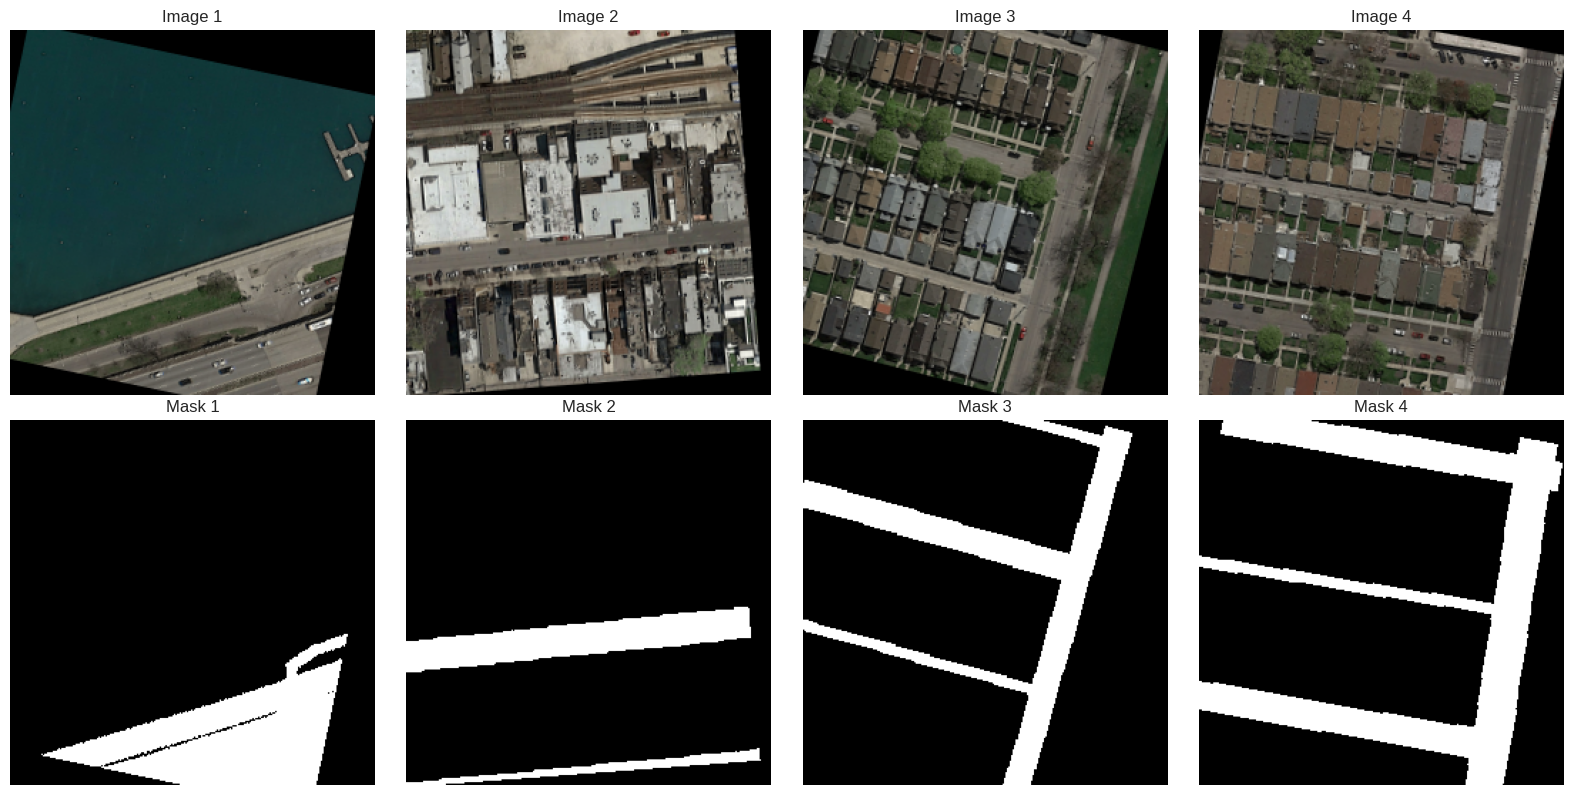
\includegraphics[width=0.95\columnwidth]{fig_dataset.png}
\caption{Dataset samples. Top: satellite images spanning urban, suburban, and rural contexts. Bottom: corresponding binary road masks with varying road density and layout complexity.}
\label{fig:dataset}
\end{figure}

\subsection{Synthetic Image Generation via Pix2Pix}

The Pix2Pix-generated images in the data set were produced by training a conditional GAN \cite{b3} on the 100 original image-mask pairs. The generator learns the mapping from binary road masks to realistic satellite textures, while the discriminator distinguishes real from generated image-mask pairs. After training, the generator receives novel road mask configurations--including new intersection patterns, road widths, and network topologies--and produces the corresponding synthetic satellite images. The input masks serve directly as the pixel-perfect ground truth, eliminating additional annotation effort. Both the synthetic images and their corresponding road masks are distributed as part of the published Kaggle dataset \cite{b17}; the masks were created by the dataset author, likely through programmatic perturbation or recombination of the original 100 masks, and served as the conditioning inputs to the Pix2Pix generator.

We assessed synthetic image quality through visual inspection of randomly sampled generated images. The generated samples exhibit realistic road surface textures, building shadows, vegetation patterns, and lighting conditions that are difficult to distinguish from the originals. Road boundary sharpness and color distributions are consistent with the real images. We retained the full generated set without filtering, as the overall quality was acceptable. Importantly, synthetic generation provides diversity that traditional augmentation (rotation, flipping, color jittering) cannot achieve: fundamentally new road layouts, intersection configurations, and background contexts that expand the distribution of training examples.

\subsection{Preprocessing and Runtime Augmentation}

The data set exhibits moderate class imbalance, with road pixels comprising 15--25\% of the image area depending on the scene. Road widths range from approximately 10 to 50 pixels. All images are resized to 256$\times$256 pixels and normalized using ImageNet statistics (mean and standard deviation per channel). We employ an 85\%--15\% training-validation split. For each random seed, this split is resampled from the available training set, while the 50-image test set remains fixed and untouched throughout training and model selection.

During training, we apply runtime augmentation with Albumentations \cite{b16} only to the training split. Augmentations include horizontal and vertical flips (probability 0.5), random rotation ($\pm$15\textdegree), shift-scale-rotate transforms, brightness and contrast adjustments ($\pm$0.2), and Gaussian noise injection. All geometric transforms are applied identically to images and their corresponding masks to preserve spatial alignment.

\section{Methodology}
\label{sec:methodology}

\subsection{Baseline U-Net Architecture}

Our baseline follows the U-Net architecture \cite{b1} adapted for binary road segmentation. The encoder consists of four sequential blocks that extract features at progressively lower spatial resolutions. Each encoder block contains a double convolution module---two consecutive 3$\times$3 convolutions, each followed by batch normalization and ReLU activation---and concludes with 2$\times$2 max pooling. The channel progression follows 3$\rightarrow$64$\rightarrow$128$\rightarrow$256$\rightarrow$512, with spatial resolution halving at each stage from 256$\times$256 to 16$\times$16.

The bottleneck operates at the lowest resolution (16$\times$16) with 1024 channels, providing a globally-aware feature representation that captures overall road network structure and spatial relationships spanning the entire image.

The decoder mirrors the encoder with four upsampling blocks. Each block uses a 2$\times$2 transposed convolution to double spatial resolution while halving the channel count. Upsampled features are concatenated with corresponding encoder features via skip connections, then processed by a double convolution module and dropout (rate 0.1) for regularization. The skip connections enable fine-grained spatial information to flow directly from encoder to decoder without passing through the information bottleneck.

A final 1$\times$1 convolution maps the 64-channel output feature map to single-channel raw logits; no sigmoid is applied at the output layer because the training loss (\texttt{BCEWithLogitsLoss}) fuses the sigmoid and the binary cross-entropy computation internally for numerical stability. The complete architecture contains 31.04 million trainable parameters.

\subsection{Attention-Gated U-Net Variant}

We enhance the baseline by incorporating attention gates \cite{b2} into each of the four skip connections. Standard skip connections pass all encoder features to the decoder indiscriminately. For road segmentation, where roads occupy a small fraction of the image, most encoder features correspond to irrelevant background (buildings, vegetation, water). Attention gates address this by learning spatial attention coefficients.

The attention gate mechanism computes a coefficient $\alpha$ for each spatial location using encoder features $\mathbf{x}$ and the decoder gating signal $\mathbf{g}$ from the next-coarser level:
\begin{equation}
\alpha = \sigma(\psi(\text{ReLU}(\mathbf{W}_x \mathbf{x} + \mathbf{W}_g \mathbf{g} + \mathbf{b})))
\end{equation}
where $\mathbf{W}_x$ and $\mathbf{W}_g$ are learned 1$\times$1 convolutions that project encoder and decoder features into a shared intermediate space, $\psi$ produces single-channel attention logits, and $\sigma$ is sigmoid activation that normalizes coefficients to $[0,1]$. The attended features $\hat{\mathbf{x}} = \mathbf{x} \odot \alpha$ replace the raw skip features, where $\odot$ denotes element-wise multiplication. Locations with high $\alpha$ (near 1) pass features unchanged; locations with low $\alpha$ (near 0) are suppressed.

The four attention gates collectively add approximately 350,000 parameters, bringing the total to 31.39M (1.1\% increase over baseline). This minimal overhead makes attention gates an efficient modification for investigating data-dependent attention effectiveness.

\subsection{Loss Function}

We employ a combined binary cross-entropy (BCE) and Dice loss:
\begin{equation}
\mathcal{L}_{total} = \mathcal{L}_{BCE} + \mathcal{L}_{Dice}
\end{equation}

Binary cross-entropy provides pixel-wise supervision, treating each pixel independently. It produces stable gradients but can be dominated by the majority class (background) under class imbalance. Dice loss directly optimizes the region overlap metric, providing supervision that is less sensitive to class imbalance by measuring the ratio of intersection to total area. The combination leverages complementary strengths: BCE provides stable per-pixel gradients while Dice loss ensures the model attends to minority-class regions (roads).

\subsection{Training Configuration}

Both architectures use identical training configurations to ensure fair comparison, isolating architectural effects from optimization differences. We use the Adam optimizer with $\beta_1$=0.9, $\beta_2$=0.999, and initial learning rate $10^{-3}$. ReduceLROnPlateau scheduling monitors validation Dice coefficient, reducing the learning rate by factor 0.5 when performance plateaus for 5 consecutive epochs (minimum lr $10^{-6}$). Batch size is 8. Training runs for a maximum of 50 epochs with early stopping at patience 10. Weight initialization follows Kaiming normal distribution. Mixed precision training (FP16) via PyTorch's GradScaler is employed for computational efficiency. Each experiment is repeated with three random seeds (42, 123, 456) to report mean $\pm$ standard deviation. The random seed affects weight initialization, data shuffling, and the training-validation split.

\subsection{Evaluation Metrics}

We evaluate using two primary overlap metrics. The Dice coefficient (equivalent to the F1 score) and Intersection over Union (IoU, Jaccard index):
\begin{equation}
\text{Dice} = \frac{2 \cdot TP}{2 \cdot TP + FP + FN}, \quad \text{IoU} = \frac{TP}{TP + FP + FN}
\end{equation}
IoU is a strictly more conservative metric than Dice for the same predictions (IoU $\leq$ Dice). Both metrics are threshold-dependent; we use the standard threshold of 0.5. We additionally compute precision, recall, and pixel accuracy for supplementary analysis.

\section{Experiments and Results}
\label{sec:experiments}

\subsection{Experimental Design}

We conduct four experiments in a 2$\times$2 factorial design crossing architecture type (Baseline U-Net, Attention U-Net) with dataset size (Original: 100 images, Extended: 1,100+ images including Pix2Pix-generated). Each experiment is run with three random seeds, yielding 12 total training runs. All experiments share identical preprocessing pipelines, runtime augmentation, and hyperparameters. Training is conducted on an NVIDIA H100 GPU using PyTorch.

\subsection{Quantitative Results}

All quantitative metrics in Tables~\ref{tab:main_results}--\ref{tab:full_metrics} are computed on the validation split (15\% of training images, resampled per seed). The held-out 50-image test set is reserved exclusively for the qualitative analysis in Section~\ref{sec:qualitative}. Table~\ref{tab:main_results} presents multi-seed results (mean $\pm$ std over 3 seeds).

\begin{table}[t]
\caption{Segmentation Performance (mean $\pm$ std, $n$=3 seeds)}
\label{tab:main_results}
\centering
\begin{tabular}{llcc}
\toprule
\textbf{Dataset} & \textbf{Model} & \textbf{Dice} & \textbf{IoU} \\
\midrule
Original & Baseline & $.7623 \pm .0921$ & $.6249 \pm .1151$ \\
(100 imgs) & Attention & $.8095 \pm .0193$ & $.6808 \pm .0272$ \\
\midrule
Extended & Baseline & $.9540 \pm .0054$ & $.9123 \pm .0100$ \\
(1,100+) & Attention & $\mathbf{.9608 \pm .0030}$ & $\mathbf{.9247 \pm .0055}$ \\
\bottomrule
\end{tabular}
\end{table}

Three key observations emerge from Table~\ref{tab:main_results}. First, Attention U-Net outperforms baseline on \emph{both} datasets when evaluated across seeds (Dice +4.7 points on original, +0.7 points on extended). Second, the standard deviations tell a striking story: on the original dataset, baseline U-Net has 4.8$\times$ higher Dice variance than Attention U-Net (0.0921 vs.\ 0.0193), indicating extreme seed sensitivity. One of the three seeds produced a baseline Dice above 0.84, while another fell below 0.70---a range that could lead to contradictory conclusions depending on which single seed is evaluated. Third, data expansion reduces variance dramatically for both models: baseline std drops from 0.0921 to 0.0054 (17$\times$ reduction), attention std from 0.0193 to 0.0030 (6$\times$).

Table~\ref{tab:improvement} quantifies the impact of data expansion versus architecture choice in absolute percentage-point (pp) differences. Data expansion improves baseline Dice by +19.17~pp and attention Dice by +15.13~pp, whereas the architecture gap is only 0.7--4.7~pp. The expansion gain dwarfs the architecture effect by roughly 4$\times$.

\begin{table}[t]
\caption{Effect Sizes: Data Expansion vs.\ Architecture}
\label{tab:improvement}
\centering
\begin{tabular}{lcc}
\toprule
\textbf{Comparison} & \textbf{Dice} & \textbf{IoU} \\
\midrule
Attn vs.\ Baseline (Orig) & +4.72 pp & +5.59 pp \\
Attn vs.\ Baseline (Ext) & +0.68 pp & +1.24 pp \\
\midrule
Baseline: Orig $\rightarrow$ Ext & +19.17 pp & +28.74 pp \\
Attention: Orig $\rightarrow$ Ext & +15.13 pp & +24.39 pp \\
\bottomrule
\end{tabular}
\end{table}

Table~\ref{tab:full_metrics} reports additional metrics confirming consistent patterns. Attention U-Net achieves higher precision and recall in both settings.

\begin{table}[t]
\caption{Supplementary Metrics (mean $\pm$ std, $n$=3 seeds)}
\label{tab:full_metrics}
\centering
\small
\begin{tabular}{llccc}
\toprule
\textbf{Data} & \textbf{Model} & \textbf{Precision} & \textbf{Recall} & \textbf{Pix.\ Acc.} \\
\midrule
Orig & Baseline & $.699 \pm .135$ & $.857 \pm .014$ & $.893 \pm .055$ \\
 & Attention & $.753 \pm .051$ & $.879 \pm .022$ & $.921 \pm .013$ \\
\midrule
Ext & Baseline & $.952 \pm .010$ & $.956 \pm .003$ & $.981 \pm .002$ \\
 & Attention & $.957 \pm .003$ & $.965 \pm .003$ & $.984 \pm .001$ \\
\bottomrule
\end{tabular}
\end{table}

\subsection{Training Dynamics}

Figs.~\ref{fig:comparison} and~\ref{fig:training_original} show training curves from a single representative seed (seed~42); all quantitative comparisons in Tables~\ref{tab:main_results}--\ref{tab:full_metrics} are multi-seed averages and should be used for performance conclusions.

Fig.~\ref{fig:comparison} illustrates performance comparison across all four experiments. On the original dataset, both models converge within approximately 20 epochs but plateau at lower performance levels. Both architectures show overfitting signs: training loss continues decreasing while validation loss stabilizes or increases. Limited data constrains achievable performance regardless of architecture.

\begin{figure}[t]
\centering
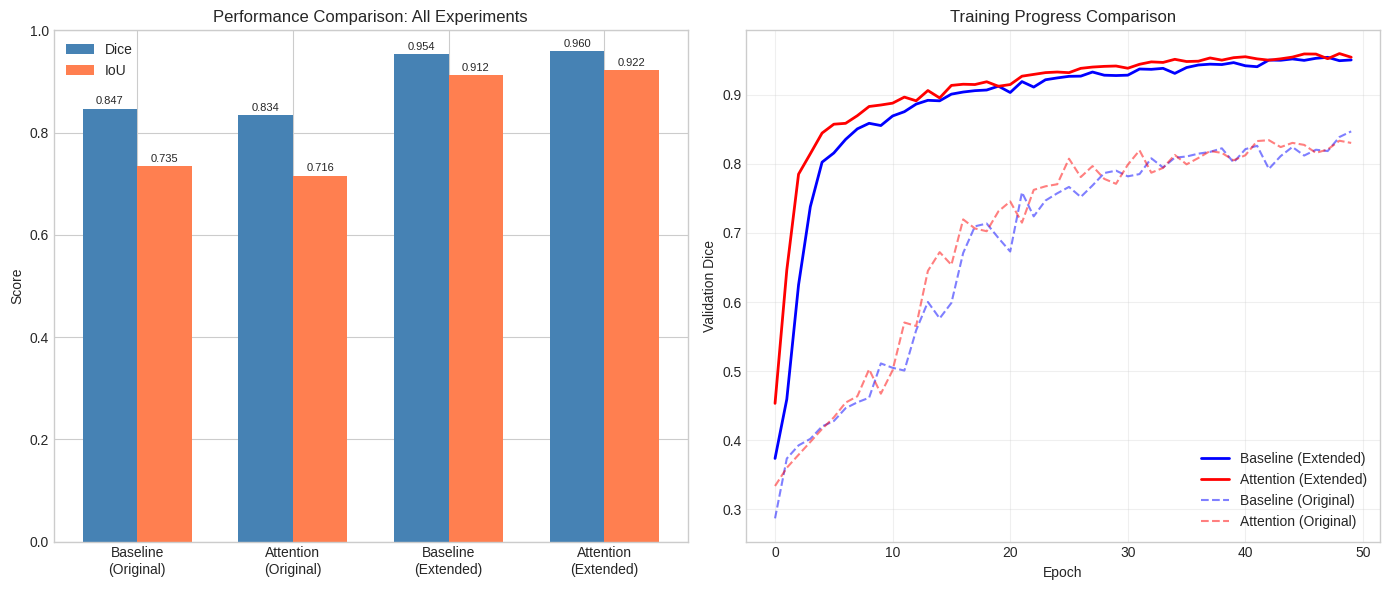
\includegraphics[width=0.95\columnwidth]{fig_comparison.png}
\caption{Performance comparison across all experiments. Left: Dice and IoU bar comparison. Right: validation curves showing substantially higher performance on extended data.}
\label{fig:comparison}
\end{figure}

On the extended dataset, both architectures achieve substantially higher performance with more stable training dynamics. The larger training set provides sufficient examples for continued improvement throughout training, with less pronounced overfitting. Attention U-Net's advantage emerges in later epochs after the attention gates have accumulated sufficient gradient signal to learn effective spatial weighting patterns.

Fig.~\ref{fig:training_original} shows training curves for original-dataset experiments. The learning rate scheduler reduces the rate when validation plateaus, but limited data constrains ultimate performance for both architectures.

\begin{figure}[t]
\centering
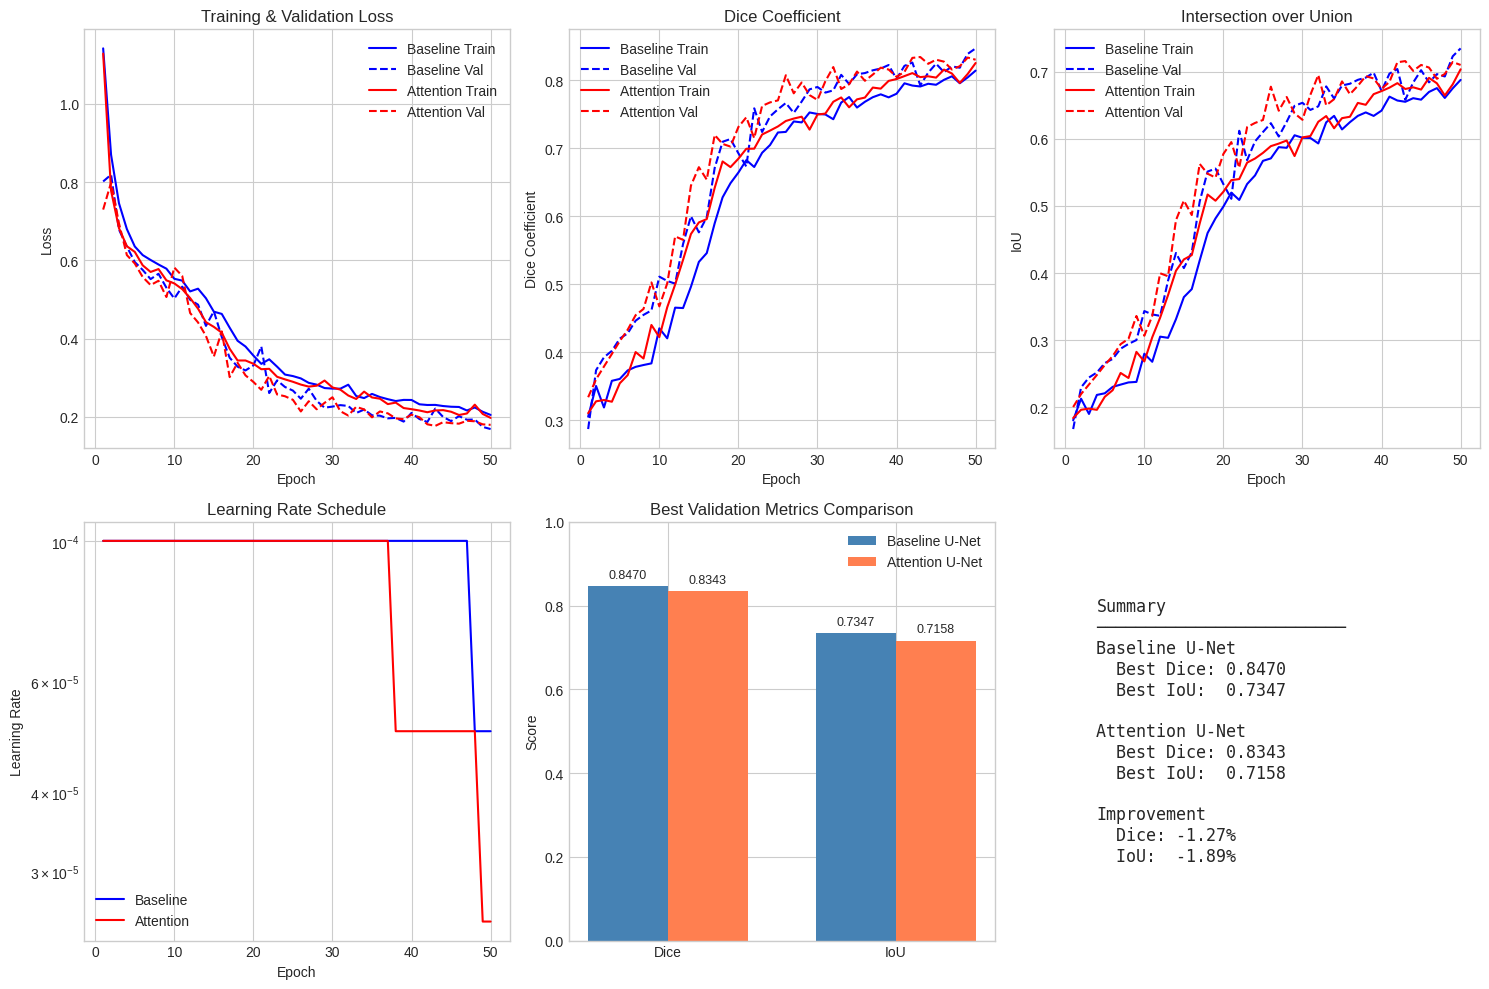
\includegraphics[width=\columnwidth]{fig_training_original.png}
\caption{Training metrics on original dataset (100 images). Both models plateau early due to limited data, with high epoch-to-epoch variance.}
\label{fig:training_original}
\end{figure}

\subsection{Qualitative and Zoomed-In Analysis} 
\label{sec:qualitative}
Fig.~\ref{fig:qualitative} compares predictions on representative validation images. Both models segment major roads well; differences are subtle and concentrated at boundaries and shadow-affected areas.

\begin{figure}[t]
\centering
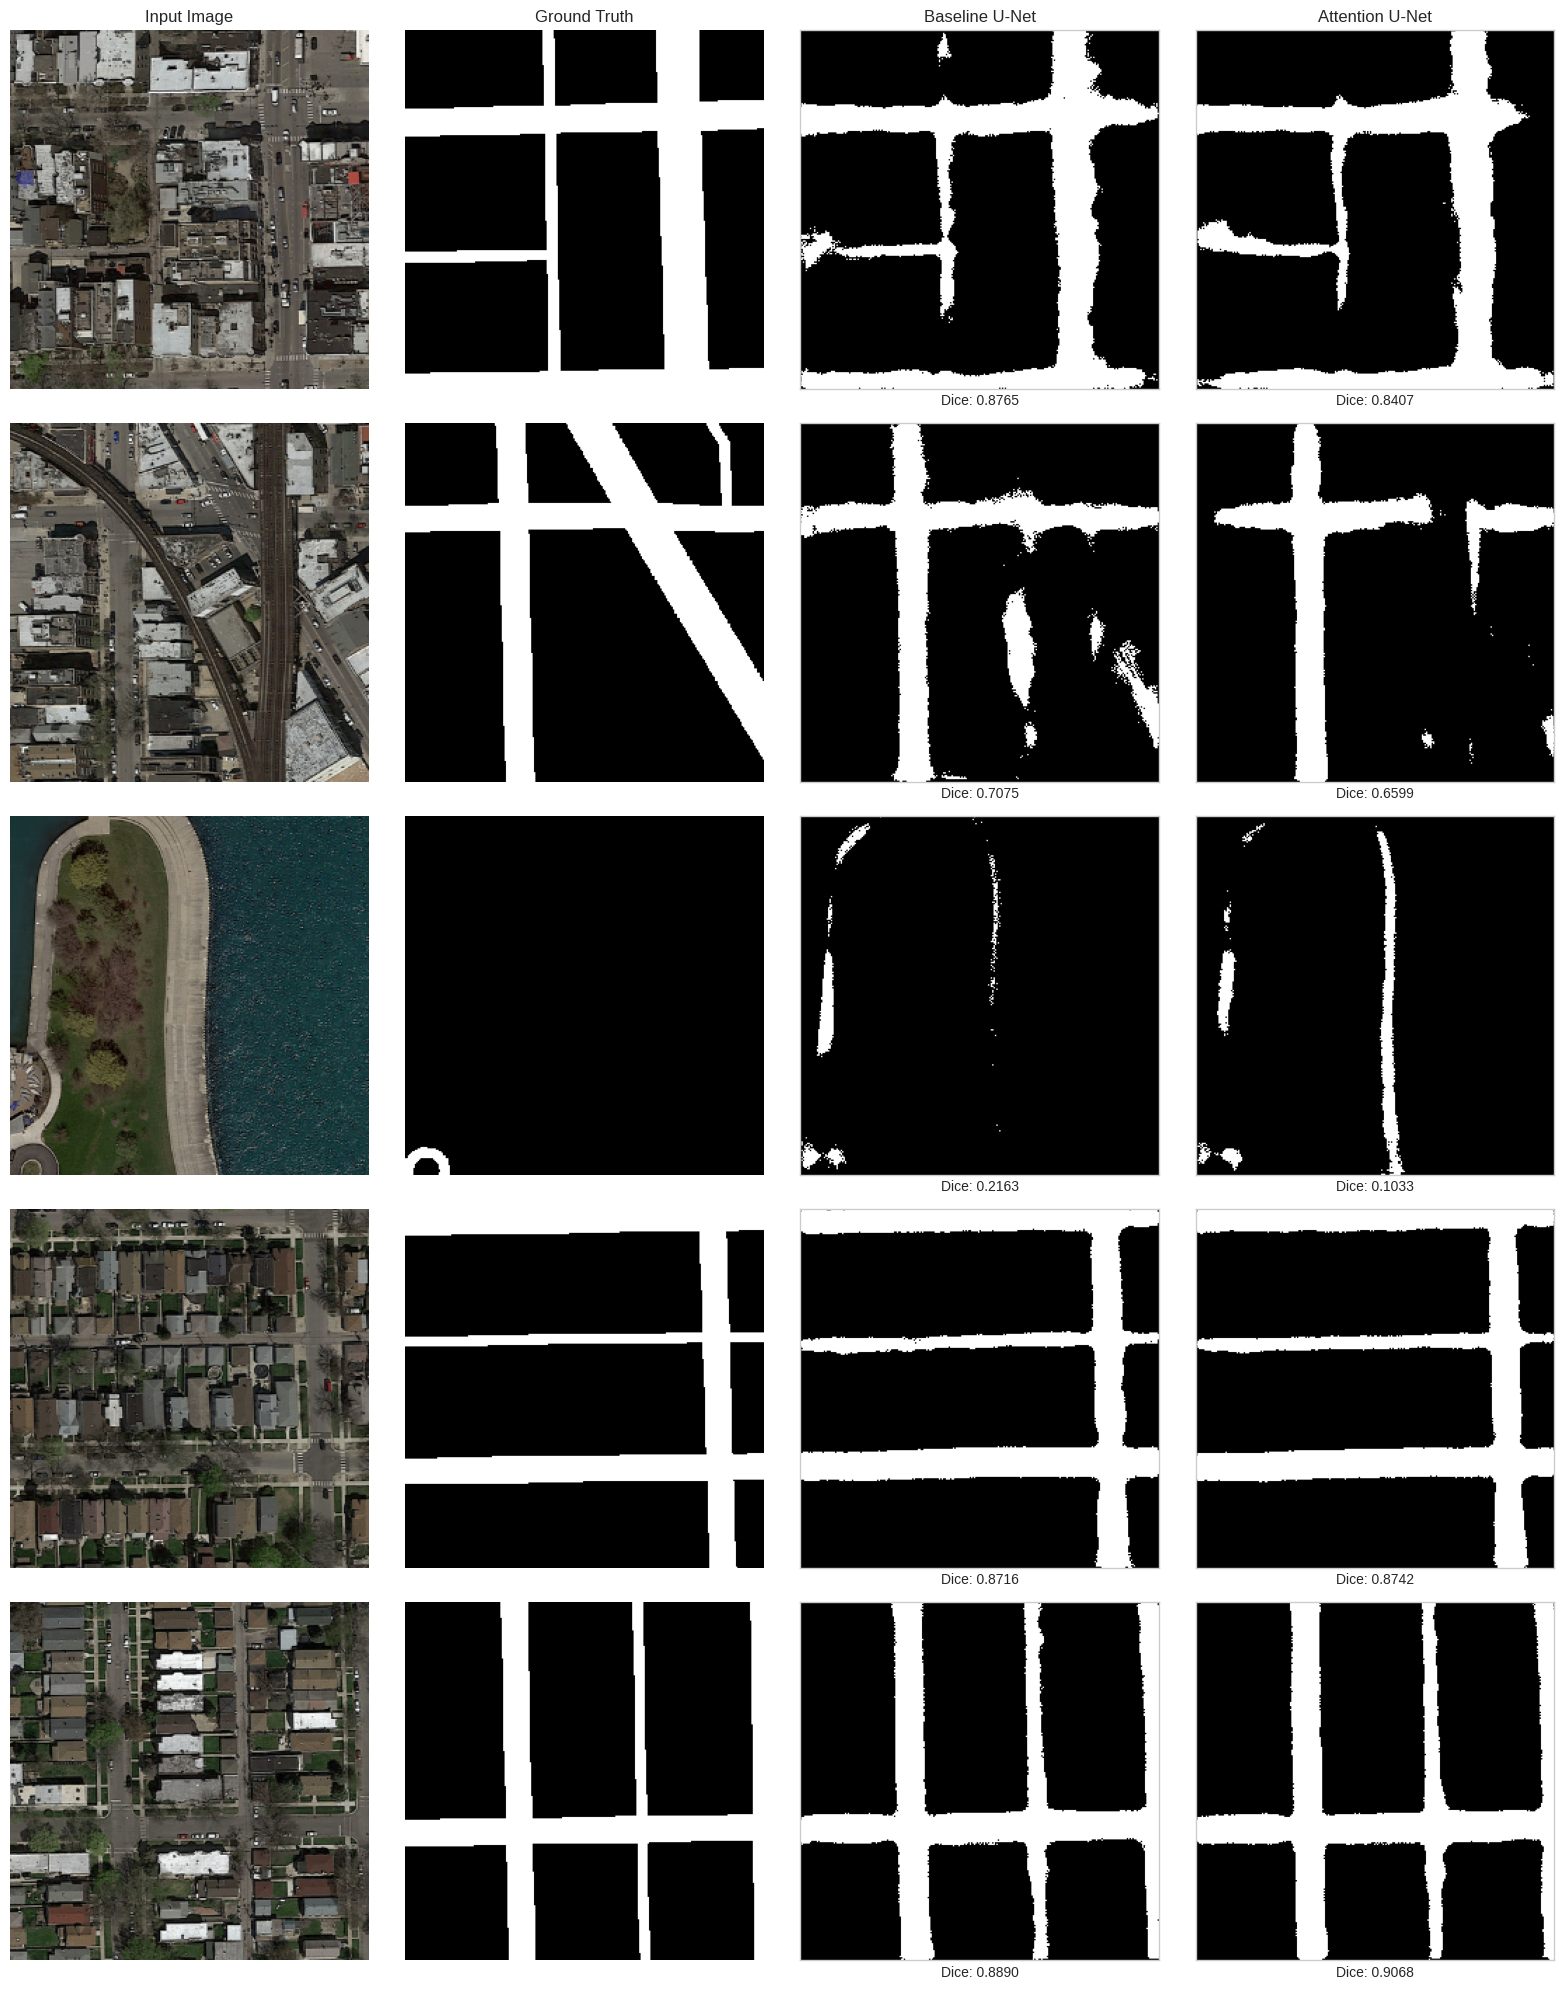
\includegraphics[width=0.85\columnwidth]{fig_qualitative.png}
\caption{Qualitative comparison on validation images. Columns: input, ground truth, baseline prediction, Attention U-Net prediction.}
\label{fig:qualitative}
\end{figure}

To identify where the models disagree, Fig.~\ref{fig:zoomed} presents zoomed-in crops of regions with maximum prediction disagreement between baseline and Attention U-Net. For each of three selected validation images (chosen as those with highest pixel-wise disagreement), we locate the spatial region of maximum disagreement and display both the full prediction comparison and a zoomed overlay crop.

The color-coded difference maps reveal systematic patterns in where the two architectures diverge. Disagreements concentrate at three types of regions: (1) road boundaries where the transition from road surface to adjacent land cover is gradual, (2) thin or narrow road segments where a few pixels of difference substantially affects the prediction, and (3) shadow-affected areas where buildings or dense vegetation cast shadows across road surfaces, reducing contrast. In these challenging regions, Attention U-Net tends to produce sharper, more decisive boundaries, while baseline U-Net occasionally over-segments (predicting road in adjacent non-road areas) or under-segments (missing portions of thin road segments). These qualitative observations are consistent with the quantitative finding that Attention U-Net achieves higher precision (0.957 vs.\ 0.952 on extended data), indicating fewer false positive road pixels.

\begin{figure}[t]
\centering
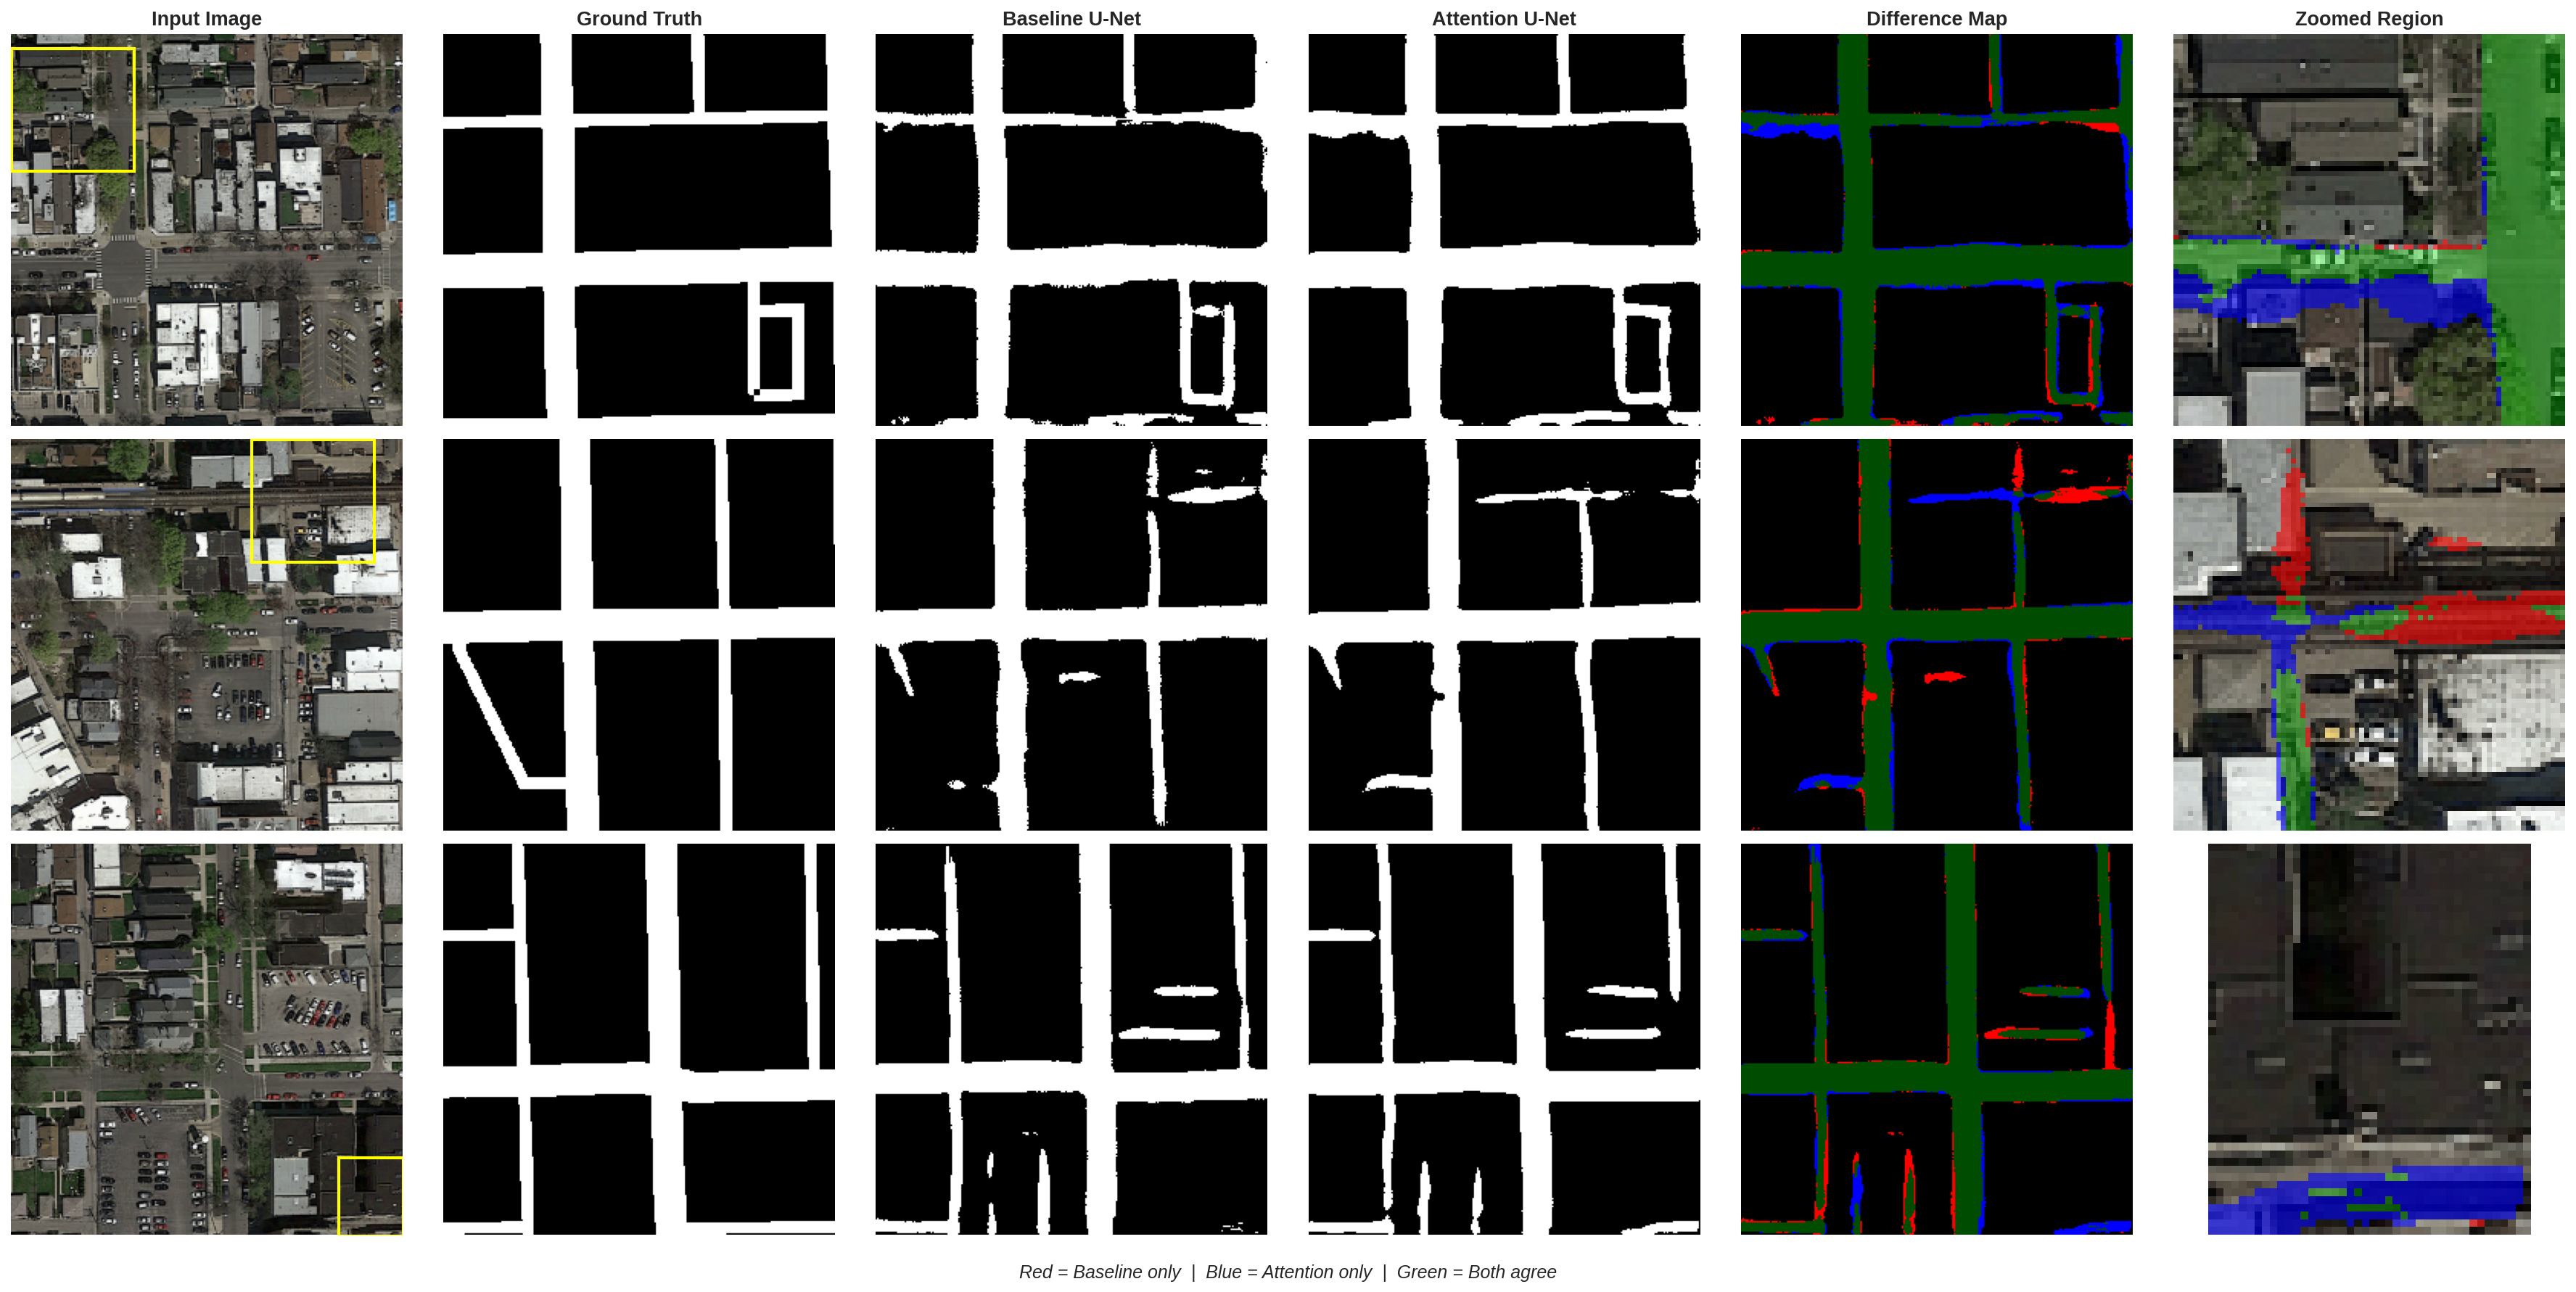
\includegraphics[width=0.95\columnwidth]{fig_zoomed_comparison.png}
\caption{Zoomed-in comparison at regions of maximum disagreement. Red: baseline-only predictions. Blue: attention-only predictions. Yellow rectangles on input images indicate zoomed regions.}
\label{fig:zoomed}
\end{figure}

\subsection{Test Set Evaluation}

Fig.~\ref{fig:test_predictions} shows predictions on the 50 held-out test images with difference maps. Overall pixel agreement is 92.89\%, with disagreements concentrated at road boundaries.

\begin{figure}[t]
\centering
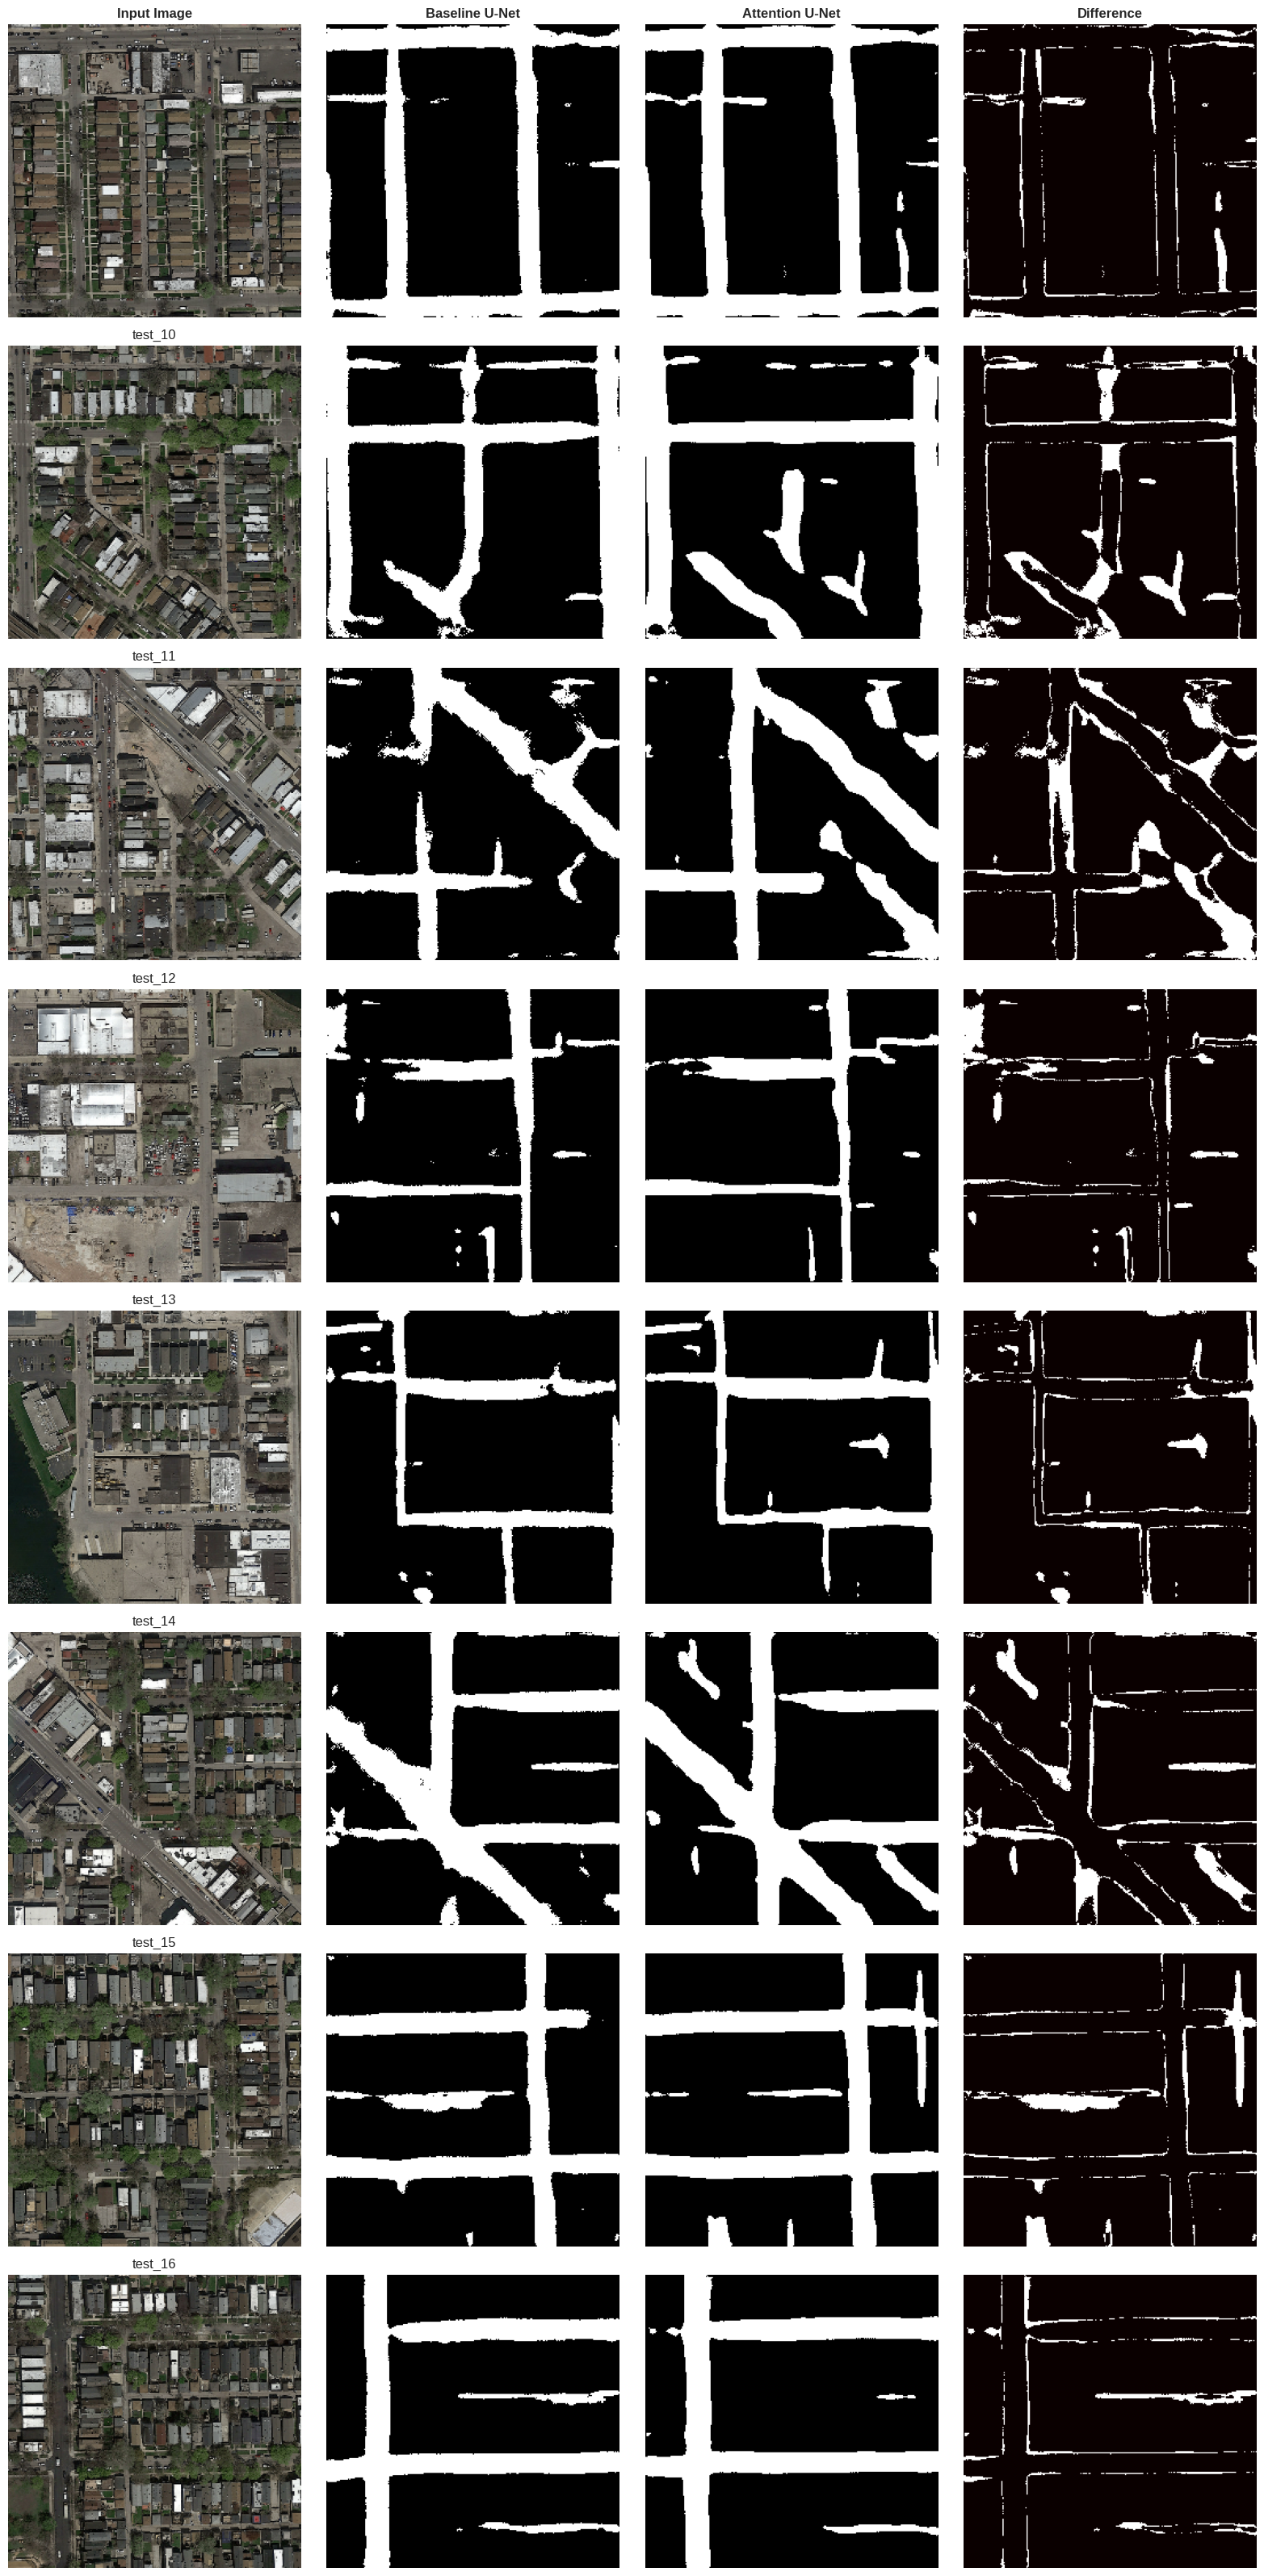
\includegraphics[width=0.95\columnwidth]{fig_test_predictions.png}
\caption{Test predictions with difference maps. White pixels indicate disagreement between models. Overall pixel agreement: 92.89\%.}
\label{fig:test_predictions}
\end{figure}

Table~\ref{tab:test_stats} summarizes road coverage statistics across all 50 test images. Attention U-Net exhibits lower standard deviation in predicted road coverage (4.89\% vs.\ 5.67\%) and a more constrained maximum (39.86\% vs.\ 50.29\%), indicating more consistent predictions and reduced tendency toward over-segmentation. The baseline's maximum of 50.29\% suggests it occasionally predicts half the image as road---a failure mode that Attention U-Net avoids, likely because the attention gates learn to suppress spurious activations in non-road regions.

\begin{table}[t]
\caption{Test Set Road Coverage Statistics (\%)}
\label{tab:test_stats}
\centering
\begin{tabular}{lcccc}
\toprule
\textbf{Model} & \textbf{Mean} & \textbf{Std} & \textbf{Min} & \textbf{Max} \\
\midrule
Baseline U-Net & 21.43 & 5.67 & 12.25 & 50.29 \\
Attention U-Net & 22.42 & 4.89 & 11.56 & 39.86 \\
\bottomrule
\end{tabular}
\end{table}

Fig.~\ref{fig:overlays} shows overlay visualizations on test images, confirming that both models produce visually accurate road extractions despite the absence of ground truth. The overlays reveal both models capture major road structures, with Attention U-Net producing slightly tighter overlays in complex intersection regions.

\begin{figure}[t]
\centering
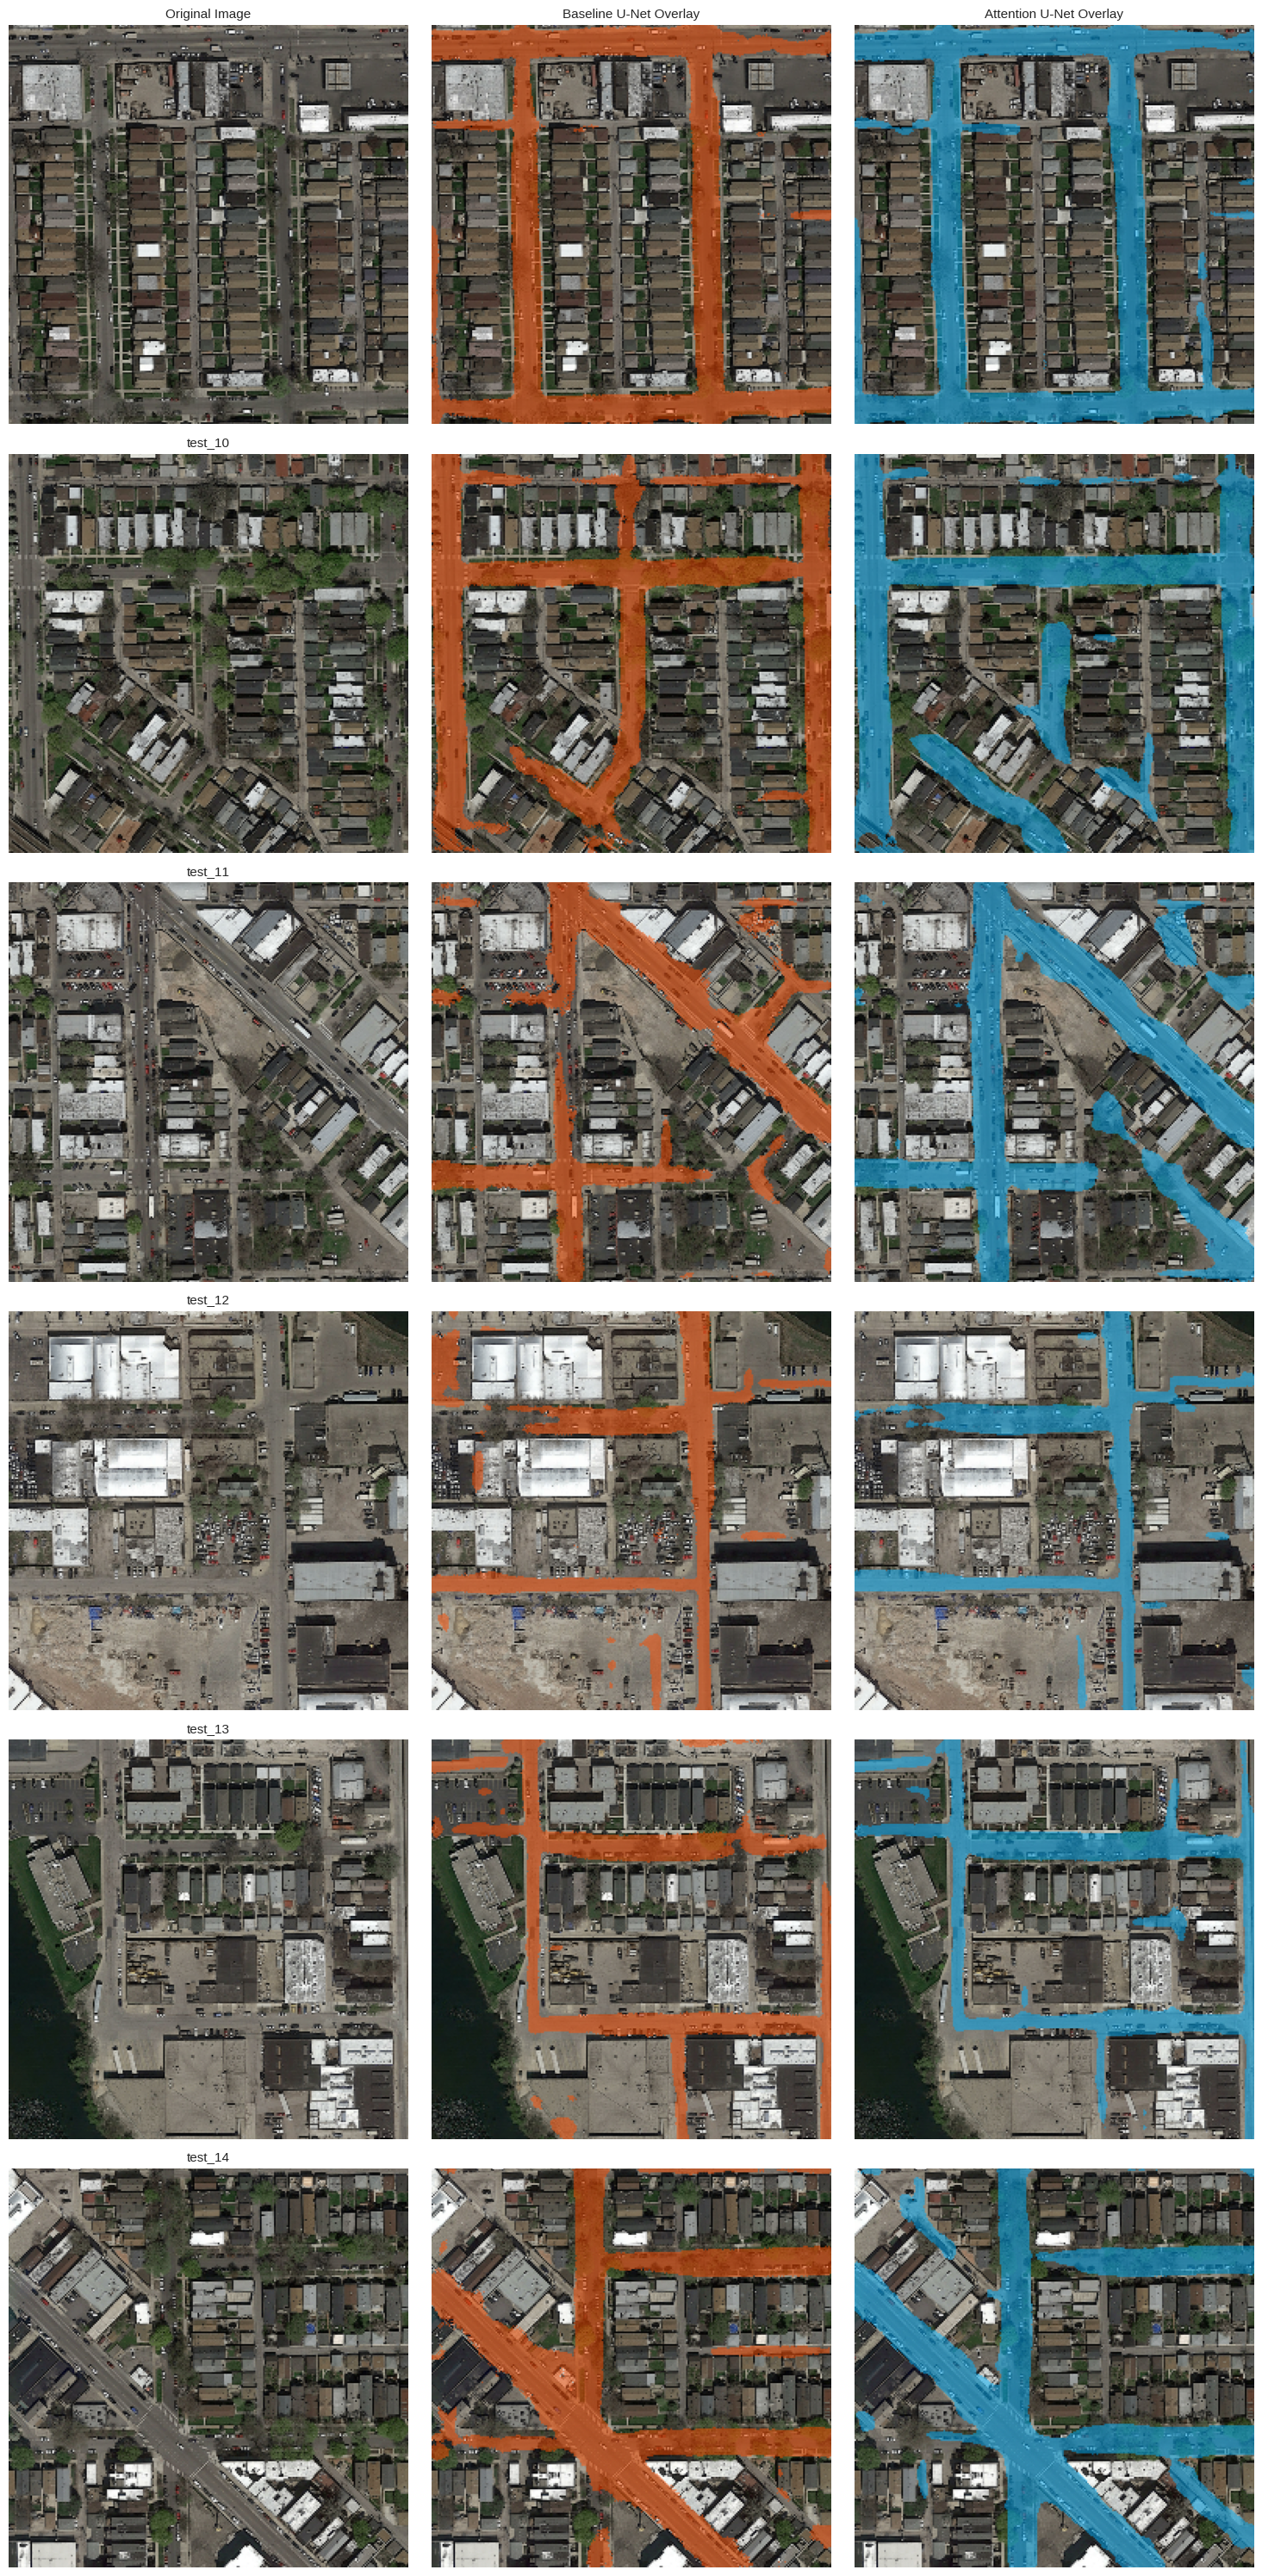
\includegraphics[width=0.95\columnwidth]{fig_test_overlays.png}
\caption{Overlay visualization on test images. Columns: original image, baseline overlay (orange), Attention U-Net overlay (blue). Both produce accurate extractions with subtle differences at intersections.}
\label{fig:overlays}
\end{figure}

\section{Discussion}
\label{sec:discussion}

\subsection{Seed Sensitivity and the Importance of Multi-Run Evaluation}

The most striking finding is the extreme seed sensitivity of baseline U-Net on limited data. With std of 0.0921 in Dice---meaning individual seeds produced results ranging from below 0.70 to above 0.84---any single-seed comparison between architectures on 100 images would be unreliable. In fact, one specific seed (42) yielded baseline Dice of 0.8470, which exceeds the attention model's mean, creating the misleading impression that baseline outperforms attention on limited data. Multi-seed evaluation reveals the opposite: Attention U-Net is both more accurate (mean Dice 0.8095 vs.\ 0.7623) and vastly more stable (std 0.0193 vs.\ 0.0921) on this small dataset.

This finding has methodological implications beyond our specific study. Architecture comparisons on small datasets that rely on a single random seed risk drawing conclusions from noise rather than signal. The random seed affects both the train/validation split (which 15 of 100 images are held out) and weight initialization, both of which can dramatically alter convergence on small datasets where each image carries disproportionate influence.

The 4.8$\times$ difference in variance between the two architectures suggests that the attention mechanism provides a regularizing effect. Attention gates constrain how encoder features are passed to the decoder, effectively reducing the space of possible feature interactions. This inductive bias appears beneficial when data is limited: it prevents the model from over-relying on spurious patterns that happen to appear in a particular train/validation split. The baseline, lacking this constraint, is free to exploit seed-specific patterns, leading to occasional high performance but also occasional poor outcomes.

The supplementary metrics in Table~\ref{tab:full_metrics} reinforce this interpretation. Baseline precision on original data shows high variance (std 0.135), meaning the model oscillates between conservative and aggressive road prediction depending on the seed. Attention U-Net's precision variance is nearly 3$\times$ lower (std 0.051), indicating more consistent decision boundaries regardless of initialization.

\subsection{Data Expansion as the Dominant Factor}

Data expansion via Pix2Pix synthesis improves baseline Dice by 19.17 absolute points and attention Dice by 15.13 points. These gains dwarf the architecture gap (0.68--4.72 points), establishing data volume as the primary performance driver on this benchmark. The baseline shows a larger absolute improvement because it starts from a lower point; attention's starting performance is already higher due to its stability advantage on limited data.

Equally important, expansion reduces variance dramatically. Baseline std drops 17$\times$ (0.0921 to 0.0054); attention std drops 6$\times$ (0.0193 to 0.0030). On the extended dataset, both models are stable across seeds and their performance gap narrows to 0.68 Dice points---a consistent but modest advantage for attention gates. The convergence in variance suggests that with sufficient data diversity, the regularizing benefit of attention gates becomes less critical, as the data itself constrains the model.

The variance reduction also has practical implications for deployment confidence. On the original dataset, a practitioner training a baseline U-Net cannot predict whether it will achieve Dice of 0.70 or 0.85---a range that could determine whether the system is deployable. With the extended dataset, both models reliably achieve above 0.95 Dice regardless of seed, providing the consistency required for production systems.

\subsection{Role of Synthetic Data}

The substantial improvements from Pix2Pix-generated images validate synthetic augmentation as highly effective for road segmentation on this dataset. Synthetic generation provides qualitatively different benefits from traditional augmentation (rotation, flipping, color jittering): it introduces fundamentally new road layouts, intersection topologies, and background contexts that expand the training distribution rather than merely perturbing existing examples. Additionally, the mask-to-image generation process ensures pixel-perfect label alignment, eliminating the annotation noise that accompanies manual labeling of additional images. We note, however, that synthetic quality was assessed through visual inspection only; quantitative fidelity metrics such as FID were not computed (see Limitations).

The variance reduction achieved through data expansion is particularly noteworthy. On the original 100-image dataset, the train/validation split determines which 15 images are held out; losing a particularly informative image to the validation set can substantially harm training. With 1,100+ images, each individual example carries proportionally less influence, naturally stabilizing outcomes across different splits.

\subsection{Practical Implications}

These results suggest a practical workflow for developing road segmentation systems: (1) prioritize expanding the training set through Pix2Pix or similar GAN-based synthesis, as data volume yields far larger gains (19+ Dice points) than architectural choice ($<$5 points on this benchmark); (2) prefer Attention U-Net over baseline even on limited data, since it is substantially more stable across seeds; (3) always report multi-seed statistics, especially when the training set is small. When budgets are limited, investment in data is more impactful than investment in model complexity.

The validation-set results reinforce this guidance. Attention U-Net's lower seed-to-seed variance (Dice std 0.0030 vs.\ 0.0054; precision std 0.003 vs.\ 0.010 on extended data) indicates that the attention mechanism produces more consistent predictions across different training conditions. Qualitative inspection of the held-out test set (Section~\ref{sec:qualitative}) corroborates this: attention predictions exhibit sharper boundaries and fewer false positives in shadow-affected and narrow-road regions.

\subsection{Limitations}

Several limitations constrain generalizability. First, all experiments use a single Kaggle satellite road dataset; results may differ across geographic regions, satellite sensors, or spatial resolutions. Second, the original dataset contains only 100 images, which inherently limits statistical power even with multi-seed evaluation---three seeds provide an indication of variance but not a rigorous confidence interval. Third, we evaluate only binary (road vs.\ background) segmentation and one attention variant (spatial attention gates on skip connections); channel attention (SE-Net), combined channel-spatial attention (CBAM), and self-attention mechanisms may exhibit different stability characteristics. Fourth, the extended-dataset performance gap (0.68 Dice points) is modest, though it is consistent across all three seeds. Finally, we assess Pix2Pix quality through visual inspection only; quantitative metrics such as Fr\'{e}chet Inception Distance could reveal systematic biases in synthetic data that might differentially affect the two architectures.

\subsection{Future Directions}

Several research directions emerge from this work. Finer-grained data volume sweeps (50, 200, 500 images) would characterize how quickly each architecture's variance decreases and performance saturates, potentially identifying an optimal data investment threshold. Comparing attention variants (SE-Net, CBAM, self-attention) under the same multi-seed factorial design would help determine whether the observed stability advantage is specific to spatial attention gates or reflects a broader property of attention mechanisms.
%would reveal whether the stability advantage we observe is specific to spatial attention gates or a general property of attention mechanisms. 
Investigating whether pretrained encoders (e.g., ResNet or EfficientNet backbones) reduce variance on small datasets could provide an alternative or complement to synthetic data expansion. Extension to multi-class road type segmentation and cross-domain evaluation across different satellite sensors would strengthen practical applicability of these findings.

\section{Conclusion}
\label{sec:conclusion}
This paper investigated an important gap in road-segmentation research: how synthetic data volume influences the observed effectiveness of attention mechanisms, and whether architecture comparisons on small datasets remain reliable under single-seed evaluation. Using a controlled multi-seed study of U-Net and Attention U-Net across limited and expanded training-data regimes, we show that reliable comparisons depend not only on mean segmentation performance but also on training stability. First, Attention U-Net consistently outperforms baseline U-Net across seeds on both limited and expanded data, but this advantage can be obscured in single-seed evaluation because the baseline exhibits substantially higher variance on the small dataset. Second, Pix2Pix-based data expansion is the dominant performance factor, improving both models by 15–19 Dice points while reducing variance by 6–17×. Third, with sufficient data, both models achieve strong performance ($>$0.95 Dice), with Attention U-Net retaining a modest but consistent advantage. In this sense, the significance of the work lies not only in the reported performance gains but also in clarifying how model comparisons should be conducted when annotated remote-sensing data are scarce: data expansion and multi-seed evaluation are essential for fair and reproducible conclusions. Although these findings are specific to the dataset, binary task, and attention variant studied, the paper provides a useful empirical framework for examining architecture–data interactions in semantic segmentation and highlights the importance of evaluating not only accuracy, but also robustness, under limited-data conditions.

\section*{Acknowledgment}

In accordance with IEEE's AI policy, the author discloses the use of Claude Opus 4.6 (Anthropic) for language editing and formatting in Sections I--VII. All experimental design, implementation, and analysis were conducted independently. References were prepared without AI assistance.

\begin{thebibliography}{00}
\bibitem{b1} O. Ronneberger, P. Fischer, and T. Brox, ``U-Net: Convolutional networks for biomedical image segmentation,'' in \emph{Proc. MICCAI}, 2015, pp. 234--241.
\bibitem{b2} O. Oktay \emph{et al.}, ``Attention U-Net: Learning where to look for the pancreas,'' in \emph{Proc. MIDL}, 2018.
\bibitem{b3} P. Isola, J.-Y. Zhu, T. Zhou, and A. A. Efros, ``Image-to-image translation with conditional adversarial networks,'' in \emph{Proc. CVPR}, 2017.
\bibitem{b4} J. Long, E. Shelhamer, and T. Darrell, ``Fully convolutional networks for semantic segmentation,'' in \emph{Proc. CVPR}, 2015.
\bibitem{b5} Z. Zhou \emph{et al.}, ``UNet++: A nested U-Net architecture for medical image segmentation,'' in \emph{Proc. DLMIA}, 2018.
\bibitem{b6} Z. Zhang, Q. Liu, and Y. Wang, ``Road extraction by deep residual U-Net,'' \emph{IEEE Geosci. Remote Sens. Lett.}, vol. 15, no. 5, pp. 749--753, 2018.
\bibitem{b7} K. He, X. Zhang, S. Ren, and J. Sun, ``Deep residual learning for image recognition,'' in \emph{Proc. CVPR}, 2016.
\bibitem{b8} J. Chen \emph{et al.}, ``TransUNet: Transformers make strong encoders for medical image segmentation,'' \emph{arXiv:2102.04306}, 2021.
\bibitem{b9} J. Hu, L. Shen, and G. Sun, ``Squeeze-and-excitation networks,'' in \emph{Proc. CVPR}, 2018.
\bibitem{b10} S. Woo, J. Park, J.-Y. Lee, and I. S. Kweon, ``CBAM: Convolutional block attention module,'' in \emph{Proc. ECCV}, 2018.
\bibitem{b11} J. Wang, N. I. R. Ruhaiyem, and P. Fu, ``A comprehensive review of U-Net and its variants,'' \emph{IET Image Process.}, vol. 19, no. 1, 2025.
\bibitem{b12} V. Mnih and G. E. Hinton, ``Learning to detect roads in high-resolution aerial images,'' in \emph{Proc. ECCV}, 2010.
\bibitem{b13} L. Zhou, C. Zhang, and M. Wu, ``D-LinkNet: LinkNet with pretrained encoder and dilated convolution for satellite road extraction,'' in \emph{Proc. CVPRW}, 2018.
\bibitem{b14} A. Batra \emph{et al.}, ``Improved road connectivity by joint learning of orientation and segmentation,'' in \emph{Proc. CVPR}, 2019.
\bibitem{b15} I. Goodfellow \emph{et al.}, ``Generative adversarial nets,'' in \emph{Proc. NeurIPS}, 2014.
\bibitem{b16} A. Buslaev \emph{et al.}, ``Albumentations: Fast and flexible image augmentations,'' \emph{Information}, vol. 11, no. 2, p. 125, 2020.
\bibitem{b17} S. Ali, ``Satellite images for road segmentation,'' Kaggle, 2023. [Online]. Available: \url{https://www.kaggle.com/datasets/sanadalali/satellite-images-for-road-segmentation}
\end{thebibliography}

\end{document}
